\subsection{Settings}
The settings subsystem allows users to changed their user account information. A user can add more music accounts (SoundCloud, Spotify, etc), logout, and change the theme.

\begin{figure}[h!]
	\centering
 	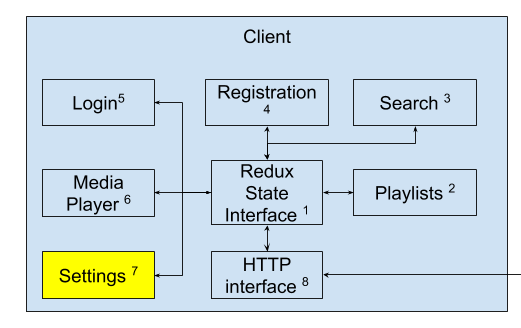
\includegraphics[width=0.60\textwidth]{images/client/client_settings.png}
 	\caption{Settings subsystem}
\end{figure}

\subsubsection{Subsystem Hardware}
No hardware is used for this layer. The setting component will be a component of the home page which will be hosted on Heroku.

\subsubsection{Subsystem Operating System}
No OS is required in order for the playlist component to work properly.

\subsubsection{Subsystem Software Dependencies}
We will be using React.js 16.8.0-alpha.1 for our framework and will be using the Fetch API from Mozilla.

\subsubsection{Subsystem Programming Languages}
We will be using JavaScript ES6

\subsubsection{Subsystem Data Structures}
A list of different configuration of Synthify that the user can use to customize their experience.

\newpage
